\chapter{The acoustic space of voice quality in Santiago Laxopa Zapotec} \label{ch:acousticlandscape}

%--------------------------------------------------------------------------
\section{Introduction} \label{sec:acousticlandscape:intro}
%--------------------------------------------------------------------------

This chapter studies the acoustic dimension of voice quality in Santiago Laxopa Zapotec (SLZ) using a Multidimensional Scaling (MDS) analysis of acoustic data. MDS is a statistical method that reduces the dimensionality of a dataset and visualizes the relationships between data points. This study uses MDS to visualize the acoustic space of voice quality in SLZ. This analysis provides information on the acoustic correlates of voice quality in SLZ and contributes to our understanding of the phonetic properties of this under-documented language.

This study is based on the work conducted by \citet{keatingCrosslanguageAcousticSpace2023} on the acoustic space of voice quality in 11 languages. However, this study focuses on a single language, SLZ, and provides a detailed analysis of the acoustic properties of voice quality in this language. The results of this study will contribute to our understanding of the phonetic properties of SLZ and how the acoustic properties of voice quality in this language compare with other languages.

%--------------------------------------------------------------------------
\section{Methods} \label{sec:acousticlandscape:methods}
%--------------------------------------------------------------------------
%--------------------------------------------------------------------------
\subsection{Participants} \label{sec:acousticlandscape:participants}
%--------------------------------------------------------------------------
This study uses data collected from 10 native speakers of SLZ during the summer of 2022. Participants were recruited from the community of Santiago Laxopa, Oaxaca, Mexico. All participants were native speakers of SLZ. The participants were between 18 and 60 years old and consisted of five males and five females.
%--------------------------------------------------------------------------
\subsection{Recordings} \label{sec:acousticlandscape:recordings} 
%--------------------------------------------------------------------------
Participants were asked to perform a word list elicitation task consisting of 72 words. These words were selected to elicit the entire range of types of voice quality in SLZ, including modal voice, the two kinds of creaky (i.e., checked and rearticulated), and breathy voice. The words were selected based on previous research conducted as part of the Zapotec Language Project at the University of California, Santa Cruz \citep{ZapotecLanguageProject}. 
Because participants were not literate in SLZ, the word list was prompted for them by asking them ``How do you say [word in Spanish]?" by myself and another researcher in Zapotec. Participants were asked to respond with the desired word in the carrier phrase \textit{Shnia' [WORD] chonhe lhas} ``I say [WORD] three times.'' which was repeated three times. These utterances were recorded in a quiet environment using a Zoom H4n digital recorder. The recordings were saved as 16-bit WAV files with a sampling rate of 44.1 kHz.

%--------------------------------------------------------------------------
\subsection{Acoustic measures} \label{sec:acousticlandscape:analysis}
%--------------------------------------------------------------------------

The resulting audio files were then processed in Praat to isolate the vowel portion of each word. The onset of the vowel was set to the second glottal pulse after the onset, and the offset of the vowel was set to the last glottal pulse before the decrease in amplitude at the end of the vowel \citep{garellekAcousticDiscriminabilityComplex2020}. The vowel was then extracted and saved as a separate file for analysis.

These vowels were fed into VoiceSauce \citep{shueVoiceSauceProgramVoice2011} to generate the acoustic measures for the studies discussed in this dissertation. Because many acoustic measures are based on the fundamental frequency, this measure was calculated using the STRAIGHT algorithm from \citep{kawaharaInstantaneousfrequencybasedPitchExtraction1998} to estimate the fundamental frequency in millisecond (ms) intervals. Once the fundamental frequency is calculated, VoiceSauce then uses an optimization function to locate the harmonics of the spectrum, finding their amplitudes.

VoiceSauce then uses the Snack Sound toolkit \citep{sjolanderSnackSoundToolkit2004} to find the frequencies and bandwidths of the first four formants, also at millisecond intervals. The amplitudes of the harmonics closest to these formant frequencies are located and treated as the amplitudes of the formants. These formant frequencies and bandwidths are used to correct the harmonic amplitudes for the filtering effects of the vocal tract, using \citeauthor{iseliAgeSexVowel2007}'s \citeyear{iseliAgeSexVowel2007} extension of the method employed by \citet{hansonGlottalCharacteristicsFemale1997}. Each vowel was measured across ten equal time intervals, resulting in 22890 data points in total. These measures were then z-scored by speaker to reduce the variation between speakers and provide a way to compare the different measures directly on similar scales.

%--------------------------------------------------------------------------
\subsection{Data processing} \label{sec:acousticlandscape:data_processing}
%--------------------------------------------------------------------------
Data points with an absolute z-score value greater than three were considered outliers and excluded from the dissertation analyzes. The Mahalanobis distance was calculated in the F1-F2 panel within each vowel category. Each data point with a Mahalanobis distance greater than six was considered an outlier and excluded from the analysis. Using the Mahalanobis distance allows us to compare the data points to the mean of the F1-F2 panel for each vowel category. The larger the Mahalanobis distance is the more deviant the data point is from the mean which in turn means that the data point was improperly tracked. This is comparable to what was done in \citet{seyfarthPlosiveVoicingAcoustics2018,chaiCheckedSyllablesChecked2022,garellekPhoneticsWhiteHmong2023}. 

Energy was excluded if it had a zero value and then logarithmically transformed to normalize its right-skewed distribution. Afterward, the resulting log-transformed energy was z-scored and any data point with a z-score greater than three was excluded. This outlier removal resulted in 1918 data points being removed. 

All data points were then z-scored by speaker to reduce the variation between speakers and provide a way to compare the different measures directly on the same scale.

The residual H1* was then calculated for the remaining data points following \citet{chaiH1H2AcousticMeasure2022}. First, a linear mixed effects model was generated with the z-scored H1* as the response variable and the z-scored energy as the fixed effect. The uncorrelated interaction of the z-scored energy by speaker was treated as random. The energy factor resulting from this linear mixed-effects model was extracted. Finally, the z-scored H1* had the product of the z-scored energy and the energy factor subtracted from it to produce the residual H1* measure. 

Once these steps were completed, the mean of each combination of phonation and speaker was taken for the fourth to seventh interval of the vowel. This is similar to what \citet{keatingCrosslanguageAcousticSpace2023} did by taking the middle of the vowel for their analysis. This choice minimizes the effect of the onset and offset of the vowel on the acoustic measures, which are more likely to be affected by the surrounding consonants and should give us the most accurate representation of the vowel quality. Because z-scores were used, this resulted in negative measures, which presents a problem for MDS analyses. To correct for this, I added the absolute value of the minimum z-score to each measure. This results in a dataset that still preserves the relative differences in the scores while providing a dataset that is all positive for the MDS analysis.

%--------------------------------------------------------------------------
\subsection{Statistical analysis} \label{sec:acousticlandscape:statistics}
%--------------------------------------------------------------------------

Multidimensional scaling analysis (MDS) is a type of dimensionality reduction to visualize the relationships between data points \citep{kruskalMultidimensionalScaling1978}. Using MDS is especially effective when many variables could contribute to the data. In the case of voice quality, this is especially warranted. 

As shown in \citet{kreimanUnifiedTheoryVoice2014,kreimanValidatingPsychoacousticModel2021,garellekAcousticDiscriminabilityComplex2020}, voice quality is psychoacoustically complex and a single measure is not enough to capture the full range of voice quality. Instead, multiple measures are required that function as cues for the different types of voice quality. For example, a vowel characterized as having a breathy voice has an elevated spectral-slope and a lower harmonics-to-noise ratio than a modal voice. A creaky voice has a lowered spectral-slope and a lowered harmonics-to-noise ratio. 

Because MDS analyses that contain many variables can result in rather unmeaningful results, I chose to focus on the speaker-by-phonation interaction. This allows us to see how speakers differ in their production of the different voice qualities. This choice to focus on speaker-by-phonation means that each speaker's production of each of the four phonation contrasts is represented as a single point in the MDS plot (e.g., one point for the first speaker's modal voice, one for their checked voice, one for their rearticulated voice, and one for their breathy voice). This is similar to what \citet{keatingCrosslanguageAcousticSpace2023} did in their study of the acoustic space of voice quality in 11 languages, except that they compared the language by voice quality interaction. Both of these interactions show us similar information. The analysis of speaker-by-phonation shows us the acoustic space within a language, while the analysis using language-by-phonation shows us the acoustic space between languages.

The MDS analysis was conducted using the \texttt{metaMDS} function in the \texttt{vegan} package \citep{oksanenVeganCommunityEcology2025} in the R programming language \citep{rcoreteamLanguageEnvironmentStatistical2024}. The Manhattan distance was used to estimate the differences between the speaker-by-phonation pairs. Because the distances are non-Euclidean, the MDS analysis was conducted using the nonmetric option.

This algorithm resulted in a solution that involves several different dimensions. The number of dimensions retained directly affects how well the original data is captured. Too many dimensions and the data are overfitted; too few, and the data are underfitted. To determine the number of dimensions to retain, I used a scree plot to plot the stress of each dimension. As shown in Figure~\ref{fig:stress_plot}, most of the data are captured in the first four dimensions. These four dimensions were retained for the analysis.

\begin{figure}[h!]
    \centering
    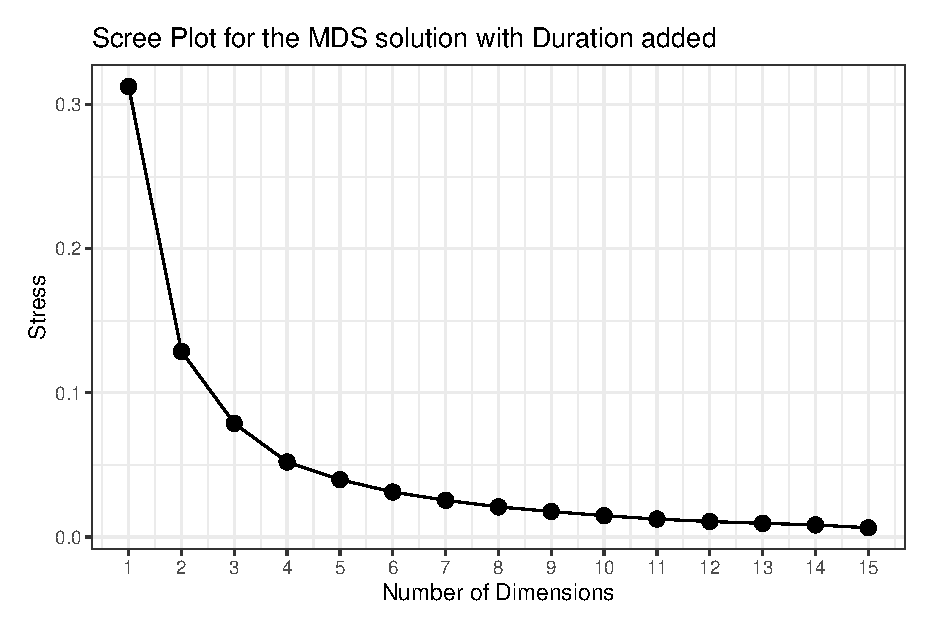
\includegraphics[width = 0.9\linewidth]{images/MDS/stress_plot_dur.eps}
    \caption{Scree plot showing the stress for each dimension for the MDS analysis.}
    \label{fig:stress_plot}
\end{figure}

% \begin{figure}[!h]
%     \centering
%     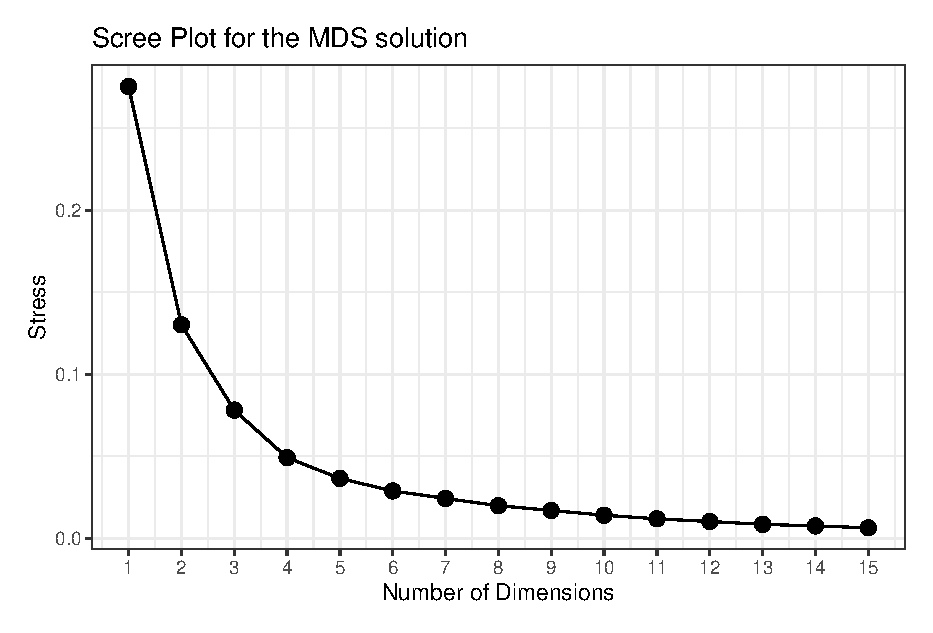
\includegraphics[width = 0.9\linewidth]{images/stress_plot_4:7.eps}
%     \caption{Scree plot showing the stress for each dimension for the MDS analysis.}
%     \label{fig:stress_plot}
% \end{figure}

%--------------------------------------------------------------------------
\section{Results} \label{sec:acousticlandscape:results}
%--------------------------------------------------------------------------
%--------------------------------------------------------------------------
\subsection{Acoustic space of voice quality} \label{sec:acousticlandscape:space}
%--------------------------------------------------------------------------

The results of the MDS analysis show that the acoustical space is represented primarily by a three-dimensional space.\footnote{A 3D plot showing the acoustic space can be found at \href{https://www.mlbrinkerhoff.me/files/3d_plot.html}{https://www.mlbrinkerhoff.me/files/3d_plot.html}.} In all subsequent plots, breathy voice is represented by orange, checked voice with blue, rearticulated voice with green, and modal voice with black. In each of the plots, the modal voice is generally more densely packed than the non-modal voice qualities. This is likely due to the fact that the modal voice represents approximately 60\% of the data, while the non-modal voice qualities represent approximately 40\% of the data.Another possible reason for this is that modal voice is more stable and less variable than the non-modal voice qualities, which would result in a more densely packed representation of the modal voice in the acoustic space. 
% The exact proportions of the data are given in Table~\ref{tab:voice_quality_proportions}.

% \begin{table}[ht]
%     \centering
%     \caption{Proportions of the different voice qualities in the dataset.} 
%     \label{tab:voice_quality_proportions}
%     \begin{tabular}{cccc}
%         \lsptoprule
%         Modal & Breathy & Checked & Rearticulated \\ 
%         \hline
%         0.62707838  &  0.14441805  &  0.09738717  &  0.13111639 \\
%         \lspbottomrule
%     \end{tabular}
% \end{table}

Figure~\ref{fig:nmds12} shows the first dimension plotted against the second dimension. In this plot, we observe that breathy voice is located in the top left of the plot, modal voice is located in the bottom center of the plot, and the two types of creaky voices are located to the right of the plot, with checked voice located at the extreme right of the plot, and rearticulated voice located closer to the center. From this plot, we see that the first dimension separates breathy, modal, and creaky voices. The second dimension separates the modal voice, bottom of the plot, from the non-modal voice qualities, top of the plot.

\begin{figure}[h!]
    \centering
    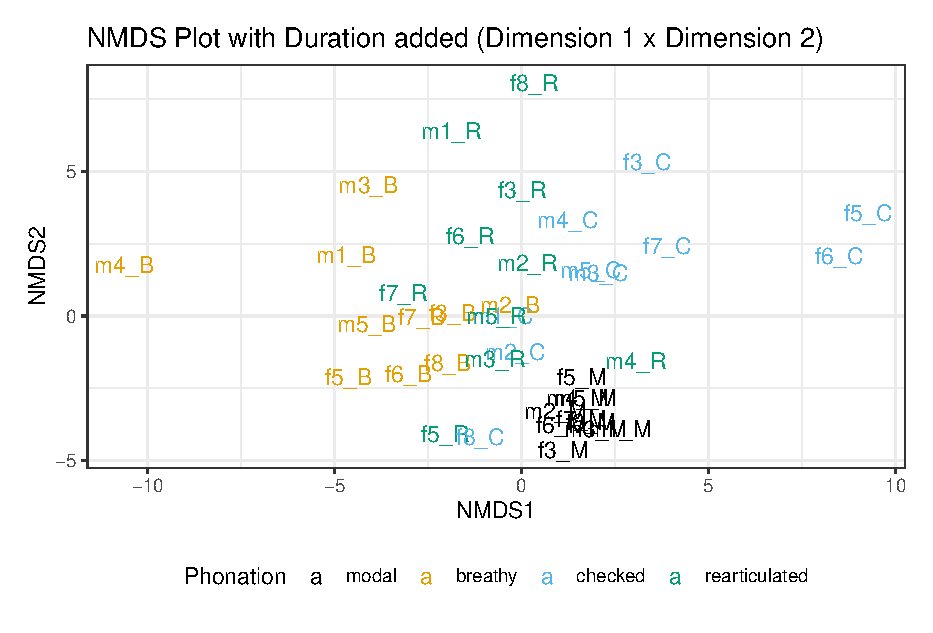
\includegraphics[width = 0.75\linewidth]{images/MDS/nmds12_dur.eps}
    \caption{Two-dimensional MDS solution showing the first and second dimensions.}
    \label{fig:nmds12}
\end{figure}

% \begin{figure}[h!]
%     \centering
%     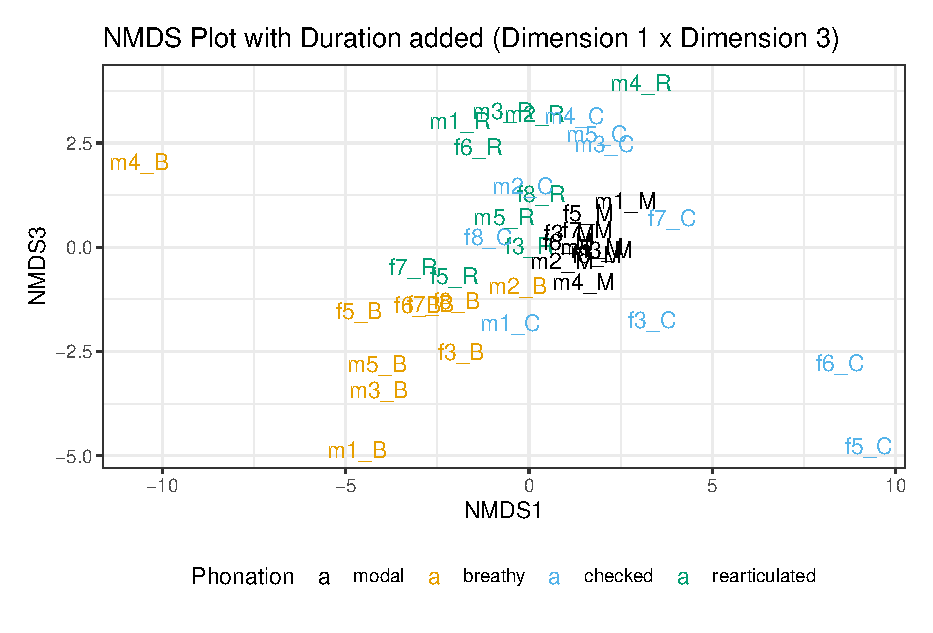
\includegraphics[width = 0.9\linewidth]{images/MDS/nmds13_dur.eps}
%     \caption{Two-dimensional MDS solution showing the first and third dimensions.}
%     \label{fig:nmds13}
% \end{figure}

Figure~\ref{fig:nmds13} compares the first dimension with the third dimension. In this plot, we observe that the breathy voice is located in the bottom left of the plot, modal voice is located in the very center of the plot, and the two types of creaky voices are located in the top right of the plot. It should be noted that the distribution of the different voice qualities follows a line from bottom left to top right in the plot. This suggests that the first and third dimensions capture similar information about voice quality in SLZ.

\begin{figure}[!h]
    \centering
    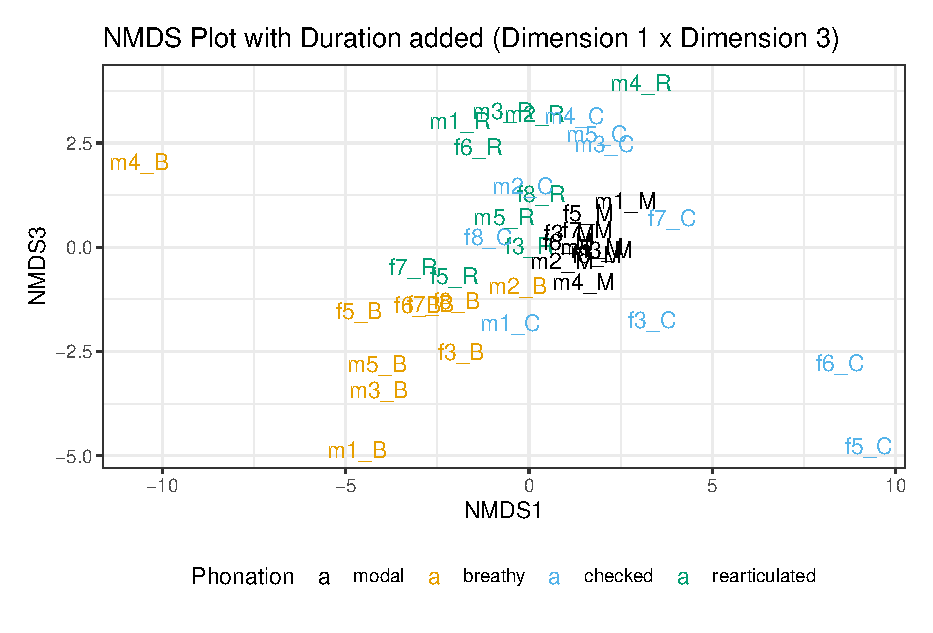
\includegraphics[width = 0.75\linewidth]{images/MDS/nmds13_dur.eps}
    \caption{Two-dimensional MDS solution showing the first and third dimensions.}
    \label{fig:nmds13}
\end{figure}

Figure~\ref{fig:nmds14} shows the first dimension plotted against the fourth dimension. This plot is very similar to Figure~\ref{fig:nmds12}, with the only difference being that the fourth dimension moves the modal voice from the bottom-center of the plot to almost the exact center of the plot.

\begin{figure}[h!]
    \centering
    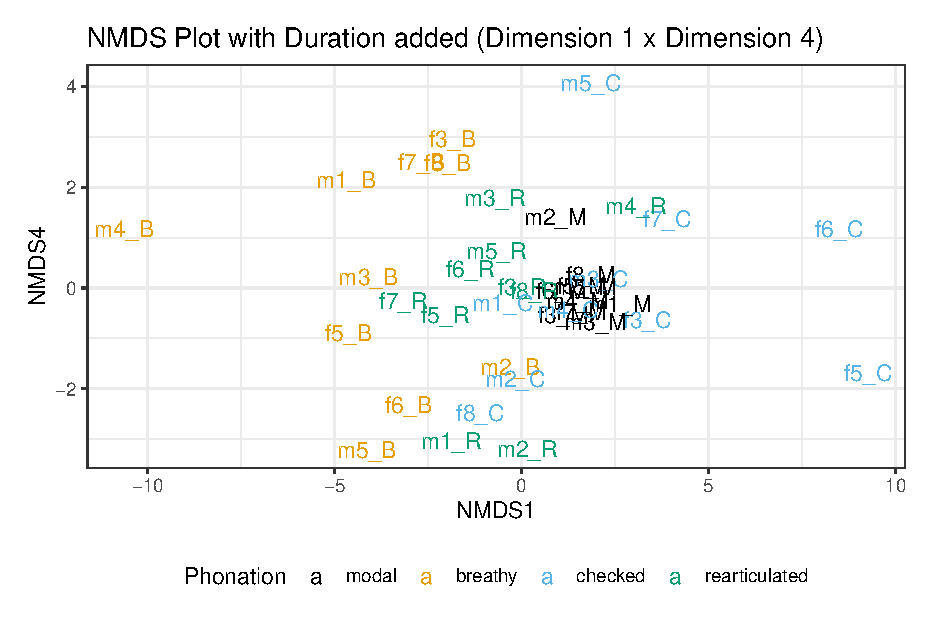
\includegraphics[width = 0.75\linewidth]{images/MDS/nmds14_dur.eps}
    \caption{Two-dimensional MDS solution showing the first and fourth dimensions.}
    \label{fig:nmds14}
\end{figure}

Figure~\ref{fig:nmds23} shows the second dimension plotted against the third dimension. This plot is essentially the same as Figure~\ref{fig:nmds13}, except that the coordinates are flipped.

\begin{figure}[h!]
    \centering
    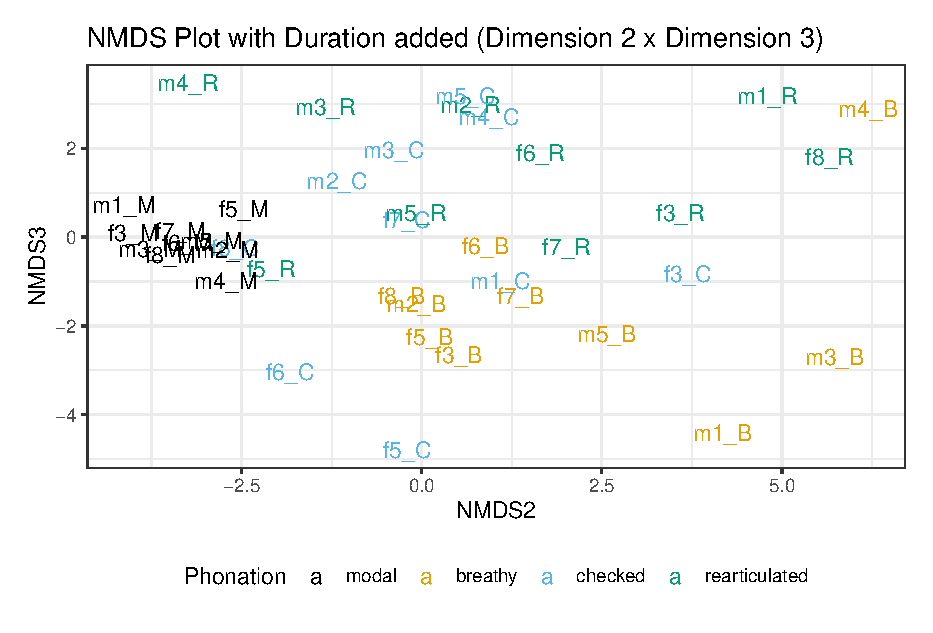
\includegraphics[width = 0.75\linewidth]{images/MDS/nmds23_dur.eps}
    \caption{Two-dimensional MDS solution showing the second and third dimensions.}
    \label{fig:nmds23}
\end{figure}

Figure~\ref{fig:nmds24} shows the second dimension plotted against the fourth dimension. This plot shows that the modal voice and the non-modal voice are separated into two different clusters, with modal voice located to the extreme left of the plot and the nonmodal voice qualities located to the right of the modal grouping. Again, as first seen in Figure~\ref{fig:nmds14}, the fourth dimension centralizes the modal voice, but no discernible pattern is observed for the other phonations.

\begin{figure}[h!]
    \centering
    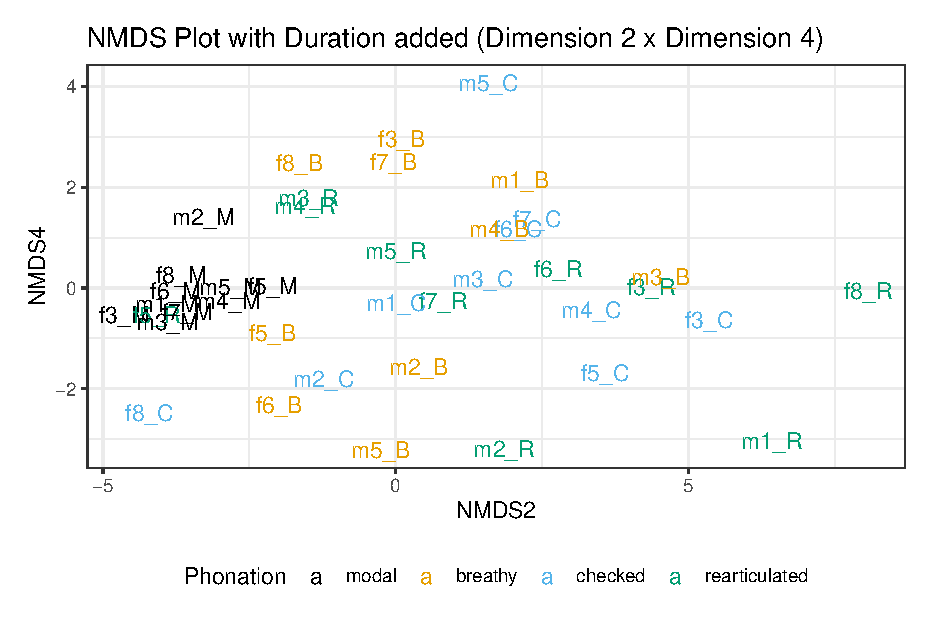
\includegraphics[width = 0.75\linewidth]{images/MDS/nmds24_dur.eps}
    \caption{Two-dimensional MDS solution showing the second and fourth dimensions.}
    \label{fig:nmds24}
\end{figure}

Figure~\ref{fig:nmds34} shows the third dimension plotted against the fourth dimension. This plot is very similar to Figure~\ref{fig:nmds14} with the exception that along the third dimension checked and rearticulated voice have swapped places. Checked voice is more centralized in the plot, whereas rearticulated voice is located more to the right of the plot. Again, we observe that the modal voice is located in the center of the plot.

\begin{figure}[h!]
    \centering
    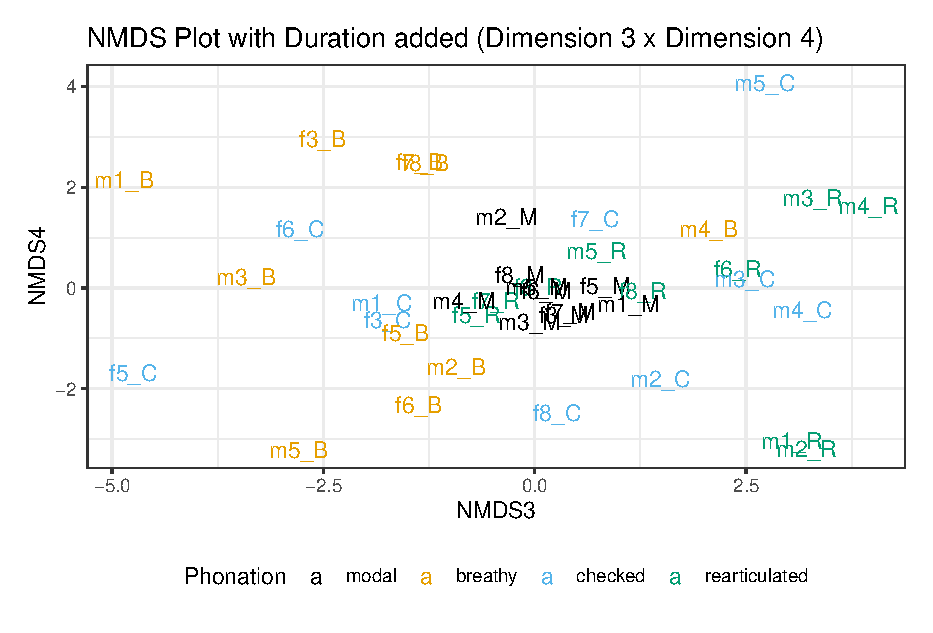
\includegraphics[width = 0.75\linewidth]{images/MDS/nmds34_dur.eps}
    \caption{Two-dimensional MDS solution showing the third and fourth dimensions.}
    \label{fig:nmds34}
\end{figure}

% From these plots, we can see that the 

%--------------------------------------------------------------------------
\subsubsection{Interim summary for dimension plots} \label{sec:acousticlandscape:inter_sum}
%--------------------------------------------------------------------------

The plots of the MDS analysis show that the acoustic space of voice quality in SLZ is primarily represented by a three-dimensional space. The first dimension and third dimensions are very similar in that they capture a continuum from breathy, to modal, and finally creaky voice. This is similar to what \citet{keatingCrosslanguageAcousticSpace2023} found in their study for the second dimension. 

This continuum from breathy to modal to creaky is very similar to the open-quotient model of voice quality proposed by \citet{gordonPhonationTypesCrosslinguistic2001}, as illustrated in Figure~\ref{fig:phonation_types}. Because of this similarity to the open-quotient model, the first and third dimensions are likely capturing the open-quotient of the glottis. 

\begin{figure}[h!]
    \centering
    \begin{tikzpicture}
        % Draw the line with arrows at both ends
        \draw[<->, line width=0.5mm] (0,0) -- (10,0);
        
        % Labels underneath the line
        \node[below] at (0,0) {[h]};
        \node[below] at (2,0) {Breathy};
        \node[below] at (5,0) {Modal};
        \node[below] at (8,0) {Creaky};
        \node[below] at (10,0) {[ʔ]};
        
        % Labels above the line
        \node[above] at (0,0) {Open Glottis};
        \node[above] at (10,0) {Closed Glottis};
    \end{tikzpicture}
    \caption{A diagram showing the relationship between breathy, modal, and creaky phonation types from \citet{gordonPhonationTypesCrosslinguistic2001}.}
    \label{fig:phonation_types}
\end{figure}

From the plots involving the second dimension, we see that this dimension separates the modals from the non-modal ones. This is similar to what we observe with the various harmonics-to-noise ratios and the cepstral peak prominence (CPP) which are all measures of the amount of noise present in the signal across various bandwidths \citep{dekromCepstrumBasedTechniqueDetermining1993,hillenbrandAcousticCorrelatesBreathy1996,blankenshipTimingNonmodalPhonation2002,ferrerriesgoWhatMakesCepstral2020}. In addition to the amount of noise, it also captures the strength of the vocal fold vibration, similar to what \citet{garellekVoicingGlottalConsonants2021} found in their study of glottal consonants and nonmodals. In their study, they found that the modal voice had the highest strength of vocal fold vibration (measured by the Strength of Excitation), while the non-modal voice had a lower strength of vocal fold vibration. This suggests that the second dimension is to capture the amount of aperiodic voicing and aspiration noise in the signal, the strength of the vocal fold vibration, or both.

The fourth dimension is less clear in terms of what it is potentially capturing. In all of the plots involving the fourth dimension, we see that modal voice is always located near the center of the plot, while the nonmodal voice qualities are located around this point depending on the patterns from the other dimensions. This suggests that the fourth dimension possibly captures something about modal voice. 

The rest of this chapter will focus on how the different acoustic measures contribute to the different dimensions of the MDS analysis. This will be followed by a general discussion of both the MDS analysis dimensions and the acoustic measures that are correlated with these dimensions. This discussion will focus on how the results of this study relate to previous work on voice quality and the implications of these results for our understanding of the acoustic space of voice quality. 

%--------------------------------------------------------------------------
\subsection{Acoustic correlates of voice quality} \label{sec:acousticlandscape:correlates}
%--------------------------------------------------------------------------

Looking at the visual representation of the dimensions is only part of the full story. In order to fully understand what is occurring, we need to determine how the acoustic measures contribute to each of the different dimensions. There are two ways to do this: (i) looking at the amount of weight each acoustic measure contributes to the different dimensions, and (ii) looking at how correlated the different acoustic measures are to the different dimensions \citep{kruskalMultidimensionalScaling1978,hastieElementsStatisticalLearning2009}. Both of these methods are useful in understanding the shape of the data. In the following discussion, I will take the second approach and look at the correlations between the different acoustic measures and the different dimensions. This is done to make the resulting discussion easier to follow.   

Table~\ref{tab:acoustic_correlates} shows the correlation score, computed by the \texttt{cor} function in R, for each acoustic measure and dimension. The four largest correlations in each dimension are in bold. The choice to bold the four largest correlations was arbitrary and was done to make it easier to discuss. Although only the four largest correlations are bolded, there are several correlations that share similar correlation values. These cases will be discussed as needed.

\begin{table}[h!]
    \centering
    \caption{Correlations for each acoustic measure to the four dimensions (NMDS1, NMDS2, NMDS3, NMDS4). The four largest correlations in each dimension are bolded.} 
    \label{tab:acoustic_correlates}
    \begin{tabular}{lrrrr}
        \lsptoprule
        Acoustic Measure & NMDS1 & NMDS2 & NMDS3 & NMDS4 \\ 
        \hline
        H1*$-$H2* & -0.221 & -0.339 & 0.031 & 0.314 \\ 
        H2*$-$H4 & -0.437 & 0.239 & \textbf{-0.689} & \textbf{-0.364} \\ 
        H1*$-$A1* & \textbf{-0.828} & 0.048 & \textbf{-0.459} & 0.044 \\ 
        H1*$-$A2* & \textbf{-0.855} & -0.067 & -0.343 & 0.114 \\ 
        H1*$-$A3* & \textbf{-0.809} & -0.218 & -0.297 & 0.126 \\ 
        H4*$-$H2k* & -0.452 & -0.598 & 0.294 & \textbf{0.366} \\ 
        H2k*$-$H5k* & 0.152 & 0.023 & 0.101 & 0.057 \\ 
        residual H1* & -0.290 & -0.443 & \textbf{-0.722} & 0.084 \\ 
        H2* & -0.157 & -0.555 & \textbf{-0.679} & 0.114 \\ 
        H4* & 0.295 & \textbf{-0.778} & 0.078 & \textbf{0.479} \\ 
        A1* & 0.756 & -0.549 & 0.092 & 0.124 \\ 
        A2* & \textbf{0.779} & -0.476 & -0.103 & 0.086 \\ 
        A3* & 0.735 & -0.416 & -0.211 & 0.093 \\ 
        CPP & -0.590 & -0.606 & 0.209 & -0.179 \\ 
        HNR < 500 Hz & -0.513 & \textbf{-0.792} & 0.152 & -0.202 \\ 
        HNR < 1500 Hz & -0.275 & \textbf{-0.799} & 0.323 & -0.290 \\ 
        HNR < 2500 Hz & -0.327 & -0.714 & 0.391 & -0.348 \\ 
        HNR < 3500 Hz & -0.446 & -0.644 & 0.393 & -0.356 \\ 
        Strength of Excitation & -0.013 & -0.741 & -0.238 & 0.145 \\ 
        SHR & 0.144 & -0.176 & 0.122 & \textbf{-0.597} \\ 
        Energy & -0.080 & \textbf{-0.793} & -0.015 & 0.341 \\ 
        Duration & -0.622 & 0.539 & 0.257 & 0.030 \\ 
        \lspbottomrule
    \end{tabular}
\end{table}

%--------------------------------------------------------------------------
\subsubsection{Dimension 1} \label{sec:acousticlandscape:dim1}
%--------------------------------------------------------------------------
From Table~\ref{tab:acoustic_correlates}, we observe that the first dimension is negatively correlated with the acoustic slope measures of H1*$-$A1*, H1*$-$A2*, and H1*$-$A3* ($r^{2} \approx -0.825$ for all three of these measures). These measures are all types of spectral tilt measures which characterizes the difference in amplitude of the fundamental and each of the first three formants. It has been noted that these measures are correlated with the open-quotient of the glottis (see \cite{garellekPhoneticsVoice2019,garellekTheoreticalAchievementsPhonetics2022} for an overview of these measures). Because these measures all capture the same information and they are all highly correlated with the first dimension, we can conclude that the first dimension is primarily concerned with the spectral slope of the signal (i.e., the open-quotient of the glottis), in particular capturing the difference in amplitude between the fundamental and the formants.

The first dimension is also positively correlated with the amplitude of the first three formants (that is, A1*, A2*, and A3*). These acoustic measures also share correlations of a similar value ($r^{2} \approx 0.75$). It is also worth noting that these amplitude measures are all used in the normalization of the spectral slope measures (i.e., H1*$-$A1*, H1*$-$A2*, and H1*$-$A3*). I believe that this fact suggests that the first dimension is primarily concerned with the spectral slope of the signal, but is also factoring in the amplitude of the formants.

%--------------------------------------------------------------------------
\subsubsection{Dimension 2} \label{sec:acousticlandscape:dim2}
%--------------------------------------------------------------------------
The second dimension is strongly correlated with the harmonics-to-noise ratio (HNR) measures. The HNR measures HNR < 500 Hz, HNR < 1500 Hz, and HNR < 2500 Hz are all negatively correlated with the second dimension ($r^{2} \approx -0.79$). These measures are all measures of the amount of noise in the signal and are used to indicate the amount of periodicity in the signal (e.g., whether something is modal or non-modal). This suggests that the second dimension is concerned with the amount of noise in the signal.

Furthermore, there are strong negative correlations with energy, which is the root mean squared energy of the acoustic signal, and the Strength of Excitation (SoE), which is defined as ``the instant of significant excitation of the vocal-tract system during production of speech'' and represents ``the relative amplitude of impulse-like excitation'' \citep[1934]{mittalStudyEffectsVocal2014}. In other words, the SoE correlates with how strongly the vocal folds vibrate during the signal with modal voice showing the strongest amount of voicing and nonmodal phonation the least. This suggests that the second dimension is also concerned with strength of the vocal-fold vibration.

The last measure that shows a strong correlation with the second dimension is the amplitude of the fourth harmonic (H4*). This measure is negatively correlated with the second dimension ($r^{2} \approx -0.78$). This measure is typically used to help normalize the amplitude of the first formant and is used in the calculation of the spectral slope measures (e.g., H2*$-$H4*).

Together, given the correlations of the HNR measures, energy, and SoE, we can conclude that the second dimension is primarily concerned with the periodicity of the signal (i.e., the amount of noise in the signal) and the strength of the vocal fold vibration.

%--------------------------------------------------------------------------
\subsubsection{Dimension 3} \label{sec:acousticlandscape:dim3}
%--------------------------------------------------------------------------
The third dimension is negatively correlated with the two spectral tilt measures H2*$-$H4* ($r^{2} \approx -0.7$) and H1*$-$A1* ($r^{2} \approx -0.46$). H2*$-$H4* has also been shown to be another spectral slope measure that can capture the differences in amplitude between different phonation types \citep{garellekPhoneticsVoice2019,garellekModelingVoiceSource2016,kreimanUnifiedTheoryVoice2014,kreimanValidatingPsychoacousticModel2021}. This suggests that the third dimension is primarily concerned with the spectral slope of the signal, similar to what we observed in the first dimension.

In addition to the spectral tilt measures, the amplitude of the fundamental, as measured by residual H1*, and the amplitude of the second harmonic (H2*) were also found to be negatively correlated with the third dimension ($r^{2} \approx -0.7$). Residual H1* is a measure that has been shown to be robust in capturing the strength of the first harmonic \citep{chaiH1H2AcousticMeasure2022,brinkerhoffUsingResidualH12025}, which was the original goal of using higher harmonics to normalize H1 \citep{fischer-jorgensenPhoneticAnalysisBreathy1968}. The amplitude of H2* is typically used to help normalize the amplitude of the first harmonic and is used in the calculation of several spectral slope measures (e.g., H1*$-$H2*, H2*$-$H4*, etc.). These correlations indicate that the third dimension is primarily concerned with spectral tilt and the amplitude of the harmonics. 

%--------------------------------------------------------------------------
\subsubsection{Dimension 4} \label{sec:acousticlandscape:dim4}
%--------------------------------------------------------------------------

In the fourth dimension, we observe that the correlations are less clear than in the previous three dimensions. The strongest correlations in this dimension with the Subharmonic-to-Harmonic ratio (SHR; $r^{2} \approx -0.60$) describe the relative strength of any subharmonics (interharmonics) in the signal \citep{sunPitchDeterminationVoice2002}. The subharmonics in the signal correspond to alternating periods in the time domain (that is, period doubling), which typically occurs in creaky voice and with broader laryngeal constrictions (see \cite{herbstPerformanceEvaluationSubharmonictoHarmonic2021} for concerns about this acoustic measure). 

The positive correlation with H4* ($r^{2} \approx 0.48$) suggests that the fourth dimension may also capture some information about the amplitude of the higher harmonics. This is also true with the positive correlation with H4*$-$H2k* ($r^{2} \approx 0.37$) and H2*$-$H4* ($r^{2} \approx 0.36$), which are both measures that capture the spectral slope of the signal. This suggests that the fourth dimension may capture information about the amplitude of the harmonics in the signal. 

%--------------------------------------------------------------------------
\subsubsection{Interim summary for acoustic correlates} \label{sec:acousticlandscape:interim_correlates}
%--------------------------------------------------------------------------

Based on the correlations observed in Table~\ref{tab:acoustic_correlates}, we can summarize the acoustic correlates of each dimension as follows: Dimension 1 captures the spectral slope of the signal, primarily through the spectral slope measures H1*$-$A1*, H1*$-$A2*, and H1*$-$A3*. This dimension appears to be related to the amount of glottal airflow (i.e., the open-quotient of the glottis). 

Dimension 2 captures the amount of noise in the signal and the strength of vocal fold vibration, primarily through the HNR measures (HNR < 500 Hz, HNR < 1500 Hz, and HNR < 2500 Hz), Energy, and Strength of Excitation. This dimension separates modal from nonmodal voice quality.

Dimension 3 captures spectral slope of the signal, through H2*$-$H4* and H1*$-$A1*, and the amplitude of the first two harmonics through residual H1* and H2*. This dimension also appears to be related to the open-quotient of the glottis. Finally, Dimension 4 captures the periodicity in the signal through SHR and also appears to capture some information about the spectral slope, as evidenced by the amplitude of the higher harmonics through H4* and H4*$-$H2k*. However, it is not entirely clear whether this dimension is primarily concerned with the spectral slope of the signal or the periodicity in the signal.

%--------------------------------------------------------------------------
\section{Discussion} \label{sec:acousticlandscape:discussion}
%--------------------------------------------------------------------------

The results of this study show that the voice quality in SLZ occupies an acoustic space, but also shows that this space is similar to what \citet{keatingCrosslanguageAcousticSpace2023} found in their study of phonation in 11 languages. However, the results of this study differ from \citet{keatingCrosslanguageAcousticSpace2023}. Instead of a two-dimensional space like in \citet{keatingCrosslanguageAcousticSpace2023}, SLZ's voice quality occupies a three-dimensional space. Despite these differences, the behavior of the dimensions is similar to that in \citet{keatingCrosslanguageAcousticSpace2023}. 

In the analysis presented in this chapter, we see that the first and third dimensions are primarily concerned with a spectral slope continuum from positive spectral slope to negative spectral slope which correlates to breathy voice to modal voice and finally to creaky voice. As extensive research has shown, the spectral slope of the signal is closely related to the open-quotient of the glottis, or in other words, how open or closed the glottis is during phonation (see \citet{garellekTheoreticalAchievementsPhonetics2022} for an overview of this history). This continuum was also found to exist in the second dimension of \citeauthor{keatingCrosslanguageAcousticSpace2023}'s \citeyear{keatingCrosslanguageAcousticSpace2023} MDS analysis. Based on \citet{keatingCrosslanguageAcousticSpace2023} and the analysis presented in this chapter, at least one of the dimensions of any acoustic space related to voice quality must correspond to the spectral slope of the signal. 

As mentioned in Section~\ref{sec:acousticlandscape:inter_sum}, the first and third dimensions of this chapter's analysis and \citeauthor{keatingCrosslanguageAcousticSpace2023}'s second dimension, bear a striking resemblance to the voice quality model proposed by \citet{gordonPhonationTypesCrosslinguistic2001}. In \citeauthor{gordonPhonationTypesCrosslinguistic2001}'s model, voice quality is described as being a single continuum based on how open or closed the glottis is during speech. The more open the glottis, the more breathy the phonation will be. The more closed the glottis, the more creaky the phonation will be. This model also claims that laryngeal consonants [h] and [ʔ] also exist along this continuum and represent the extreme ends of this continuum.  This model can be visually represented as a line with [h] on one end and [ʔ] on the other end. The various voice qualities exist between these two extremes, as represented in Figure~\ref{fig:phonation_types_1}.

\begin{figure}[h!]
    \centering
    \begin{tikzpicture}
        % Draw the line with arrows at both ends
        \draw[<->, line width=0.5mm] (0,0) -- (10,0);
        
        % Labels underneath the line
        \node[below] at (0,0) {[h]};
        \node[below] at (2,0) {Breathy};
        \node[below] at (5,0) {Modal};
        \node[below] at (8,0) {Creaky};
        \node[below] at (10,0) {[ʔ]};
        
        % Labels above the line
        \node[above] at (0,0) {Open Glottis};
        \node[above] at (10,0) {Closed Glottis};
    \end{tikzpicture}
    \caption{A diagram showing the relationship between breathy, modal, and creaky phonation types. Based on \citet{gordonPhonationTypesCrosslinguistic2001}.}
    \label{fig:phonation_types_1}
\end{figure}

As mentioned above, the measures that correlate the most with the first dimension are several spectral slope measures (i.e., H1*$-$A1*, H1*$-$A2*, H1*$-$A3*). These correlations provide further support that the first dimension of the MDS analysis is concerned with the state of the glottis during phonation \citep{holmbergComparisonsAerodynamicElectroglottographic1995,kreimanMeasuresGlottalSource2007,garellekModelingVoiceSource2016,garellekPhoneticsVoice2019,chaiH1H2AcousticMeasure2022}.

The second dimension of this chapter's analysis is concerned with dividing the acoustic space into modal and nonmodal voice qualities. This split between modal and nonmodal is similar to the split that exists for periodicity and strength of voicing. The more modal the voice quality is, the greater the amount of periodicity or voicing that we observe in the signal. I propose that this dimension is concerned with how harmonic the signal is, or in other words, how much noise is present in the acoustic signal. This is similar to what \citet{keatingCrosslanguageAcousticSpace2023} found in their study, where the first dimension of their analysis was primarily concerned with making the same split in the acoustic space. Based on these results, I propose that another dimension in the acoustic space of voice quality must correspond to the amount of noise in the signal. This proposal is further supported by the fact that the second dimension of this chapter's analysis is primarily correlated with the harmonics-to-noise ratios, energy, and SoE measures, which are all measures of the amount of noise or the amount of energy present in the acoustic signal. 

The third dimension is similarly concerned with the spectral slope of the signal, as evidenced by the correlations with H2*$-$H4* and H1*$-$A1*. However, it is also concerned with the amplitude of the first two harmonics, as evidenced by the correlations with residual H1* and H2*. This dimension is similar to the first dimension in that it captures a spectral slope continuum from breathy to modal to creaky voice. However, it is different in that it captures not only the spectral slope of the signal, but also the amplitude of the first two harmonics. This suggests that the third dimension is primarily concerned with the spectral slope of the signal, but also captures some information about the amplitude of the harmonics in the signal.

The fourth dimension is less clear in terms of what it is capturing. The strongest correlation in this dimension is with the subharmonics-to-harmonic ratio (SHR), which suggests that this dimension may be capturing some information about the periodicity of the signal. However, there are also correlations with the amplitude of the higher harmonics (H4* and H4*$-$H2k*), which suggests that this dimension may also be capturing some information about the spectral slope of the signal or the amplitude of the these higher harmonics. However, there is no easily describable pattern that emerges with this dimension. 

The results of this study show that the voice quality acoustic space in SLZ is primarily represented by a three-dimensional space. However, it can primarily be broken down into two aspects that the acoustic space is attempting to capture: (i) the spectral slope of the signal and (ii) the amount of noise in the signal. This can be represented as a primarily two-dimensional space with higher dimensions adding additional information related to these two primary concerns. This can be visualized as a two-dimensional space with the first dimension representing the spectral slope of the signal and the second dimension representing the amount of noise in the signal, as shown in Figure~\ref{fig:acoustic_space}.

\begin{figure}[h!]
    \centering
    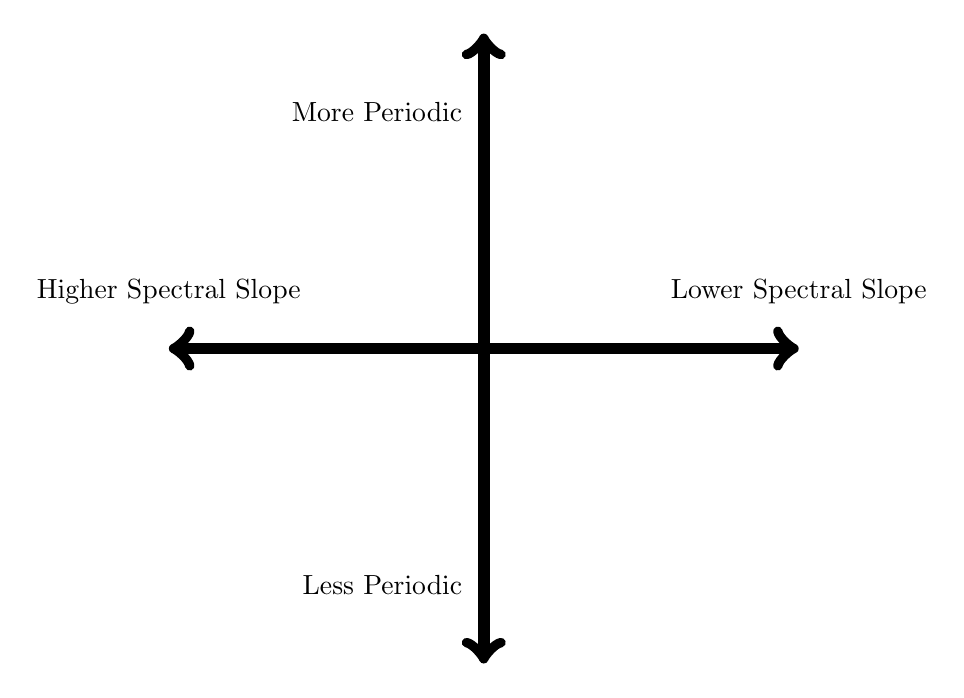
\begin{tikzpicture}
        % Draw the horizontal line with arrows
        \draw[<->, line width=1.5mm] (-4,0) -- (4,0);
        % Draw the vertical line with arrows
        \draw[<->, line width=1.5mm] (0,-4) -- (0,4);
        
        % Labels for the horizontal line
        \node[below,yshift=1cm] at (-4,0) {Higher Spectral Slope};
        \node[below,yshift=1cm] at (4,0) {Lower Spectral Slope};
        
        % Labels for the vertical line
        \node[left, xshift = -1.5mm] at (0,-3) {Less Periodic};
        \node[left, xshift = -1.5mm] at (0,3) {More Periodic};
    \end{tikzpicture}
    \caption{A two-dimensional representation of the acoustic space of voice quality in SLZ. The horizontal axis represents the spectral slope of the signal, while the vertical axis represents the amount of noise or energy in the signal.}
    \label{fig:acoustic_space}
\end{figure}

%--------------------------------------------------------------------------
\section{Conclusion} \label{sec:acousticlandscape:conclusion}
%--------------------------------------------------------------------------

Although the discussion has predominately been about the correlations of the measures that contribute to the different dimensions, it is important to note that the measures are not independent of each other. Instead, all of the measures contribute to the acoustic space of voice quality in SLZ to some extent or another. Just because a measure has a low correlation does not mean that it does not contribute to the acoustic space. Rather than thinking of the measures as independent of each other, it is better to think of them as a group of measures that work together to create the acoustic space of voice quality in SLZ. This is especially true given the fact that the MDS analysis is a reduction of the data to a few dimensions. This analysis offers a snapshot of the voice quality acoustic space in SLZ, but is not the full picture. 

In addition to the MDS analysis presented in this chapter, it is also important to consider how SLZ fits into the larger picture of voice quality in other languages. In order to see how SLZ fits in this cross-linguistic acoustic space,, we can convert the data from this analysis into a format that can be compared with the data from \citet{keatingCrosslanguageAcousticSpace2023}. This will allow us to see how SLZ fits into the larger picture of voice quality in other languages. It is expected that SLZ should pattern similarly to the other Zapotec language found in \posscitet{keatingCrosslanguageAcousticSpace2023} study. This will be addressed in a future study, as it is outside the scope of this chapter.

Furthermore, as will be discussed in Chapter~\ref{ch:revealing_trees}, another way in which we can determine which measures are the most important is by performing a classification and regression tree analysis \citep{breimanClassificationRegressionTrees1986,breimanBaggingPredictors1996,breimanRandomForests2001}.